On peut maintenant décider quelles variables supplémentaires nous ajouterons dans notre modèle. Voici la liste des variables ajoutées:

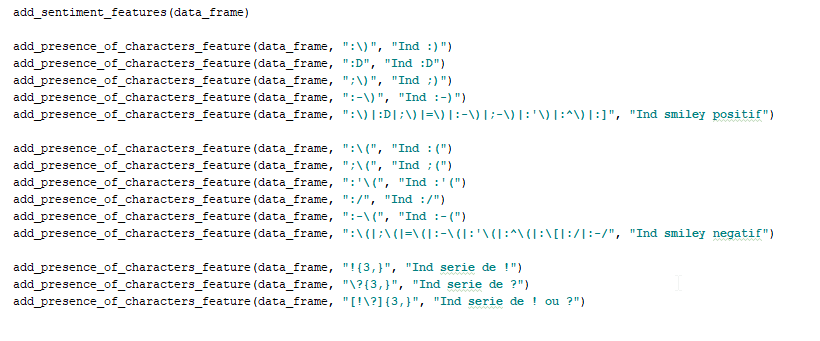
\includegraphics[width=\linewidth,height=14cm]{images/variables_autres}

La fonction \verb|add_sentiment_features| ajoute les 3 variables de sentiments, la fonction \verb|add_presence_of_characters_feature| ajoute un 1 si l'expression régulière donnée en argument est trouvée dans l'échange de textos, 0 sinon. Ainsi, les variables de sentiments, des indicateurs de \emph{smileys} positifs, négatifs et de séries de ponctuations sont ajoutés comme variables.

En conclusion, lorsqu'on roule le code avec \verb|bool_ajouter_autres_features=True|, on ajoute les variables décrites ci-dessus et on transforme tous les \emph{emojis} en texte.